\chapter{Rendre le domicile sensible au contexte}\label{cha:fiabilite} 
\begin{preamble}
Ce chapitre présente une approche visant à assurer la fiabilité de la sensibilité au contexte pour les applications d'assistance domiciliaire. 
Cette approche consiste à rendre explicite un {\em modèle de rôles} joué par les capteurs, à travers des règles, contribuant à assurer que le fonctionnement du capteur correspond à son rôle. Ces {\em règles de conformités} permettent de fournir des instructions détaillées quant à l'installation et le positionnement de capteurs dans le monde physique et assurer la conformité d'une installation déployée par rapport à son modèle durant son exploitation\footnotemark{}\footnotetext{Ce travail à fait l'objet d'une publication~:~\fullcite{carteron2016improving}.}.
\end{preamble}
\chpsummary{Contributions}
{
  Une approche qui améliore la fiabilité des applications sensibles au contexte pour la surveillance d'activité.;
  Un concept de {\em modèle de rôles de capteurs} est introduit pour capturer les besoins des applications en terme de capteurs, et permet de vérifier en continu l'infrastructure de capteurs en parallèle de l'exécution des applications.;
  Ce modèle de rôles de capteurs peut être {\em factorisé} entre les applications, {\em partagé} entre les intervenants, et {\em utilisé} pour les évolutions de la plate-forme.
}

Dans un domicile équipé d'informatique ubiquitaire, la sensibilité au contexte 
permet à une application de notifier l'utilisateur à propos d'une 
activité~\paulcite{chan2008review}, {\em uniquement} si l'activité a été 
oubliée~; elle permet de déclencher une alerte pour une porte restée ouverte 
{\em uniquement} si il n'y a personne dans la zone~; elle permet d'appeler 
l'utilisateur lorsque la cuisinière est restée allumée, {\em uniquement} 
si elle n'est pas surveillée depuis un certain temps.
La sensibilité au contexte devient alors une clé essentielle pour que ces 
applications puissent être intégrées à la vie
quotidienne de l'utilisateur. En effet, 
des notifications issues de reconnaissances de contexte erronées fatiguent 
l'utilisateur et ralentissent, voire empêchent l'acceptation de la technologie.
Il est donc essentiel de minimiser les faux positifs dans la détection de 
situations nécessitant l'attention de l'utilisateur. 

La fiabilité d'une application ubiquitaire et sensible au contexte est définie 
par la fiabilité du système dans son 
ensemble~\paulciteseparate{stankovic2005opportunities,mennicken2014from}. 
En informatique ubiquitaire, le système est principalement constitué d'une 
couche logicielle et d'une couche matérielle. 
La fiabilité logicielle a été amplement étudiée~; des approches à base de 
simulation ont été proposées~\paulcite{bruno2009diasim} pour tester la 
fiabilité du logiciel avant son déploiement. Ces approches permettent de tester,
in-vitro, des scénarios sur des applications, en simulant les interactions de 
l'utilisateur avec son environnement (\eg une ouverture de porte, une présence 
dans une pièce, la mise en marche d'un appareil). Malgré la rigueur et 
l'exhaustivité que permet la mise en {\oe}uvre de cette phase de test, la 
fiabilité logicielle reste dépendante de la fiabilité de la couche matérielle 
elle-même, fournissant les données de contexte.

La fiabilité de la couche matérielle d'un système dépend de nombreux facteurs. 
D'un point de vue unitaire, la fiabilité de la détection d'un contexte relève de la fiabilité du capteur sous-jacent. 
Elle peut être assurée simplement en vérifiant que le capteur fonctionne 
correctement. Cependant, pour être sensible au contexte, une application 
peut avoir besoin de combiner des données en provenance de plusieurs 
capteurs~\paulcite{stankovic2005opportunities}. Conceptuellement, un 
capteur est vu comme jouant un {\em rôle} dans la logique applicative~: il mesure 
les interactions des utilisateurs avec leur environnement. Ainsi, le capteur est 
supposé être placé de façon appropriée (orientation, fréquence d'échantillonnage, absence d'interférences, \etc) 
pour mesurer efficacement ces 
interactions~\paulcite[-2.8cm]{edward2011athome}. 
Quand la caractérisation d'un contexte dépend d'une combinaison d'interactions, 
le développeur construit un modèle implicite de rôles %qui doivent être 
joués par une combinaison de capteurs~\paulcite[-1.54cm]{henricksen2002modeling}. 
Par exemple, un capteur de contact sur la porte d'entrée peut
être couplé avec un capteur de mouvement couvrant la zone de l'entrée. 
Une application peut utiliser cette paire de capteurs comme suit~: si la 
porte d'entrée est restée ouverte pendant un certain temps, mais que la présence de l'utilisateur est détectée 
à proximité pendant tout ce temps, alors aucune alerte ne doit être envoyée. Cependant, il y a
certaines dépendances entre les capteurs couplés, dues au fait qu'une porte ne
s'ouvre jamais toute seule. Ces dépendances font partie du modèle implicite construit
par le développeur. Si ce modèle implicite 
est transgressé par une défaillance du capteur de mouvement, l'application 
sensible au contexte est compromise. Il peut en résulter une notification erronée 
alertant d'une situation de porte d'entrée ouverte et non surveillée, et ce, 
même si l'utilisateur est a proximité.

Pour adresser la fiabilité des capteurs, le développeur 
introduit généralement du code pour tester la validité de ce modèle implicite. Cette 
stratégie consiste à retranscrire des {\em règles implicites} via des 
instructions conditionnelles réparties à travers le code de l'application. 
Ces règles contribuent à assurer que la lecture des capteurs est conforme au 
modèle implicite. Par exemple, si une cuisine est équipée d'un capteur de contact 
sur un certain placard dans la cuisine et d'un capteur de mouvement dans la cuisine, alors, la porte du 
placard ne doit pas être détectée comme étant ouverte sans la détection 
préalable d'une présence dans la cuisine. Si cette situation se produit, 
alors il y a transgression du modèle implicite. De nombreuses raisons peuvent 
être la cause de cette violation (placement, dysfonctionnement) et doivent conduire à 
une intervention pour résoudre le problème. Détecter ces situations est un 
élément essentiel de la fiabilité des applications d'informatique ubiquitaires 
sensibles au contexte déployées dans un domicile~\paulcite{beckmann2004some}.

\section{Étude de cas}\label{seq:fiabilite:cas}
Pour illustrer notre approche, nous présentons, comme étude de cas, la 
surveillance de deux activités de cuisine. Ces exemples sont simples mais complets. 
Ils utilisent différents types de capteurs pour reconnaître différents types 
d'interactions entre l'utilisateur et son environnement dans la cuisine.

La surveillance d'activité est extrêmement dépendante de la population ciblée 
par les applications d'assistance~\paulcite{durick2013dispelling}. 
Par exemple, une personne âgée peut simplement avoir besoin d'un rappel pour la 
réalisation de ses activités quotidiennes~\paulcite{caroux2014verification}, 
alors qu'une population avec déficience intellectuelle (\eg syndrome de Down) 
peut avoir besoin de supervision pour l'exécution d'étapes clés d'une tâche~\paulcite{lussierdesrochers2016analysis}.

Pour déterminer {\em quelles} activités doivent être surveillées et {\em comment} 
elles doivent être surveillées, nous avons besoin d'expertise sur la population 
ciblée. Des professionnels comme des ergonomes et des ergothérapeutes 
fournissent cette expertise. Dans notre exemple, un expert définit les activités 
qui doivent être surveillées dans la cuisine. À partir de cet ensemble d'activités, 
l'expert détermine {\em quelles interactions} avec l'environnement doivent être 
détectées pour identifier ces activités. Typiquement, l'expert demande à 
l'utilisateur de simuler les différentes étapes effectuées pour réaliser son 
activité~\paulcite{caroux2014verification}. Une fois que les interactions 
clés concernant chaque activité d'intérêt ont été identifiées, nous devons 
déterminer {\em quels capteurs} sont pertinents pour mesurer ces interactions. 
Cette étape a été étudiée par Beckmann~\etal~\parencite{beckmann2004some}. 
Ils présentent un guide pratique pour installer les capteurs et l'évaluent à 
travers une étude utilisateurs.

Supposons maintenant que l'expert définit les activités suivantes~: (1) la 
surveillance de la préparation du petit déjeuner, pour envoyer un rappel à 
l'utilisateur si cette activité a été manquée et (2) la surveillance de la 
cuisinière pour s'assurer de son utilisation en toute sécurité.

\subsection{Surveillance de la préparation du petit déjeuner}
Pour surveiller la préparation du petit déjeuner, l'expert du domaine définit 
des scénarios typiques réalisés par l'utilisateur. 
Un de ces scénarios peut par exemple être décrit ainsi~: l'utilisateur (1) fait 
du café en utilisant une machine à café électrique, (2) prend une tasse depuis 
un placard spécifique ou le lave-vaisselle, et (3) prend du lait dans son frigidaire. 
À partir de ce scénario, il est possible d'extraire les interactions à 
mesurer~: (1) allumer la machine à café, (2) ouvrir la porte du placard, 
(3) ouvrir la porte du frigidaire. Pour mesurer ces interactions, un capteur de 
consommation électrique est associé à la machine à café~: si une consommation 
électrique est captée, alors la machine à café est allumée. Les interactions 
avec la porte du frigidaire sont détectées au moyen d'un 
capteur de contact. Pour simplifier nous n'avons pas placé de capteur de 
contact sur le lave-vaisselle, et supposons que dans ce cas, l'action de prendre 
une tasse ne peut pas être détectée.

\subsection{Sécurité de l'utilisation de la cuisinière}
Le signalement des problèmes de sécurité liés à la cuisinière dépend principalement de la détection de son 
utilisation et de la présence d'un utilisateur à proximité pour surveiller 
la cuisson. Un capteur de consommation électrique est utilisé pour détecter 
si la cuisinière est en fonctionnement, et un capteur de mouvement est positionné pour 
détecter une présence dans un périmètre stratégique autour de la cuisinière 
(typiquement l'ensemble la cuisine).

\subsection{Rendre explicite un modèle implicite}
Pour résumer, les activités à surveiller dans notre cas d'utilisation 
sollicitent la reconnaissance de cinq interactions avec l'environnement de la 
cuisine~: 
ouvrir la porte d'un placard spécifique, 
ouvrir la porte du frigidaire, 
allumer la machine à café, allumer la cuisinière, et détecter la présence dans 
la cuisine.

Pour schématiser, dans le contexte de notre cas d'utilisation, la dernière 
étape de notre méthode consiste à rendre explicite le modèle implicite qui 
assure la fiabilité des interactions détectées. Nous savons qu'un capteur de
mouvement couvre l'ensemble de la cuisine, donc, chacune des 
interactions mesurées dans la cuisine doit être précédée par la détection 
d'une présence. 
Ainsi, si une interaction est mesurée sans être 
précédée par la détection d'une présence dans la cuisine, 
%on peut supposer
il est probable 
que les capteurs impliqués ont un dysfonctionnement. Ces règles contribuent 
à assurer qu'une infrastructure de capteurs fonctionne en conformité avec 
le modèle de rôles.

\section{Besoins des applications}\label{seq:fiabilite:besoinapp}
Les applications de support d'activité domiciliaire fournissent des services 
de surveillance et d'assistance pour un utilisateur. Ces services reposent sur 
un ensemble de données contextuelles relatives à des mesures d'interactions de 
l'utilisateur avec son environnement, comme illustré avec notre cas d'étude.

Cependant, il y a souvent un fossé entre les données brutes, fournies par les 
capteurs, et le point de vue conceptuel du développeur d'applications sur 
les interactions avec l'environnement. Par exemple, un capteur de contact produit des 
valeurs booléennes définissant les états ouvert/fermé. Cet état doit être 
combiné avec l'emplacement spécifique (et/ou un identifiant) du capteur pour 
rendre l'interaction exploitable par l'application. De plus, plusieurs capteurs 
combinés peuvent être requis pour détecter une interaction. Par exemple, la 
détection d'une présence dans une pièce en forme de L nécessite plusieurs 
capteurs de mouvements.

\subsection{Rôle}
Du point de vue de l'application, le rôle définit les informations d'interaction 
directement exploitables par la logique applicative. Ce rôle consiste en un type 
d'interaction (\eg présence) et l'emplacement de l'interaction (\eg la cuisine). 
D'un point de vue physique, un rôle définit les besoins qui doivent être 
satisfaits par un ou plusieurs capteurs pour détecter une certaine interaction. 
Conceptuellement, les rôles sont positionnés entre la couche physique des 
capteurs et les applications, comme représenté en Figure~\ref{fig:appreqrole}. 
Pour être en conformité avec un rôle, les capteurs doivent être disposés 
correctement en terme de position et d'orientation. 
Comme illustré précédemment, détecter une présence dans une cuisine en forme de L 
nécessite au moins deux détecteurs de mouvements, orientés de façon à couvrir 
entièrement la cuisine, sans pour autant détecter les mouvements des espaces 
adjacents (\eg le couloir adjacent à la cuisine). Il est à noter que les rôles 
permettent la séparation des préoccupations entre les applications et la couche 
physique des capteurs.

\begin{figure}[!h]
  \centering
  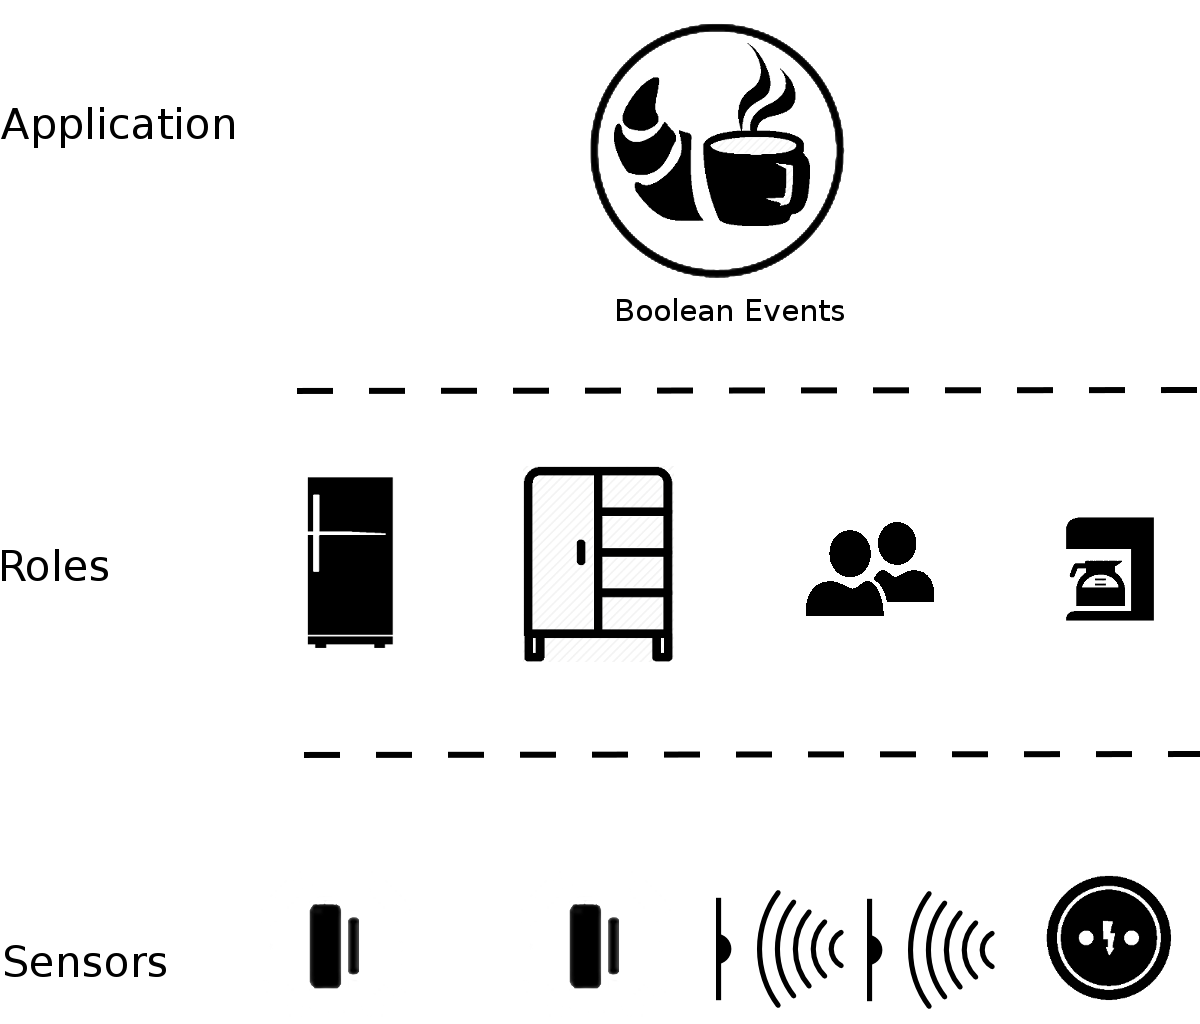
\includegraphics[width=\linewidth,totalheight=\textheight,keepaspectratio]{gfx/Roles_etc.png}
  \caption{Besoins d'application et rôles.}
  \label{fig:appreqrole}
\end{figure}

\subsection{Sémantique des rôles}
La sémantique d'un rôle couvre (1) la détection d'une interaction avec 
l'environnement, produisant une valeur {\em true}, et (2) la détection de la fin 
de cette interaction, produisant une valeur {\em false}. Ce comportement est 
illustré dans la Figure~\ref{fig:semofroles}. Un rôle est alors une fonction 
définie sur le temps et couvrant des valeurs booléennes. Quand une interaction 
est détectée à un instant, celle-ci produit true, jusqu'à ce qu'elle ne soit 
plus détectée, alors elle produit false.

\begin{figure}[!h]
  \centering
      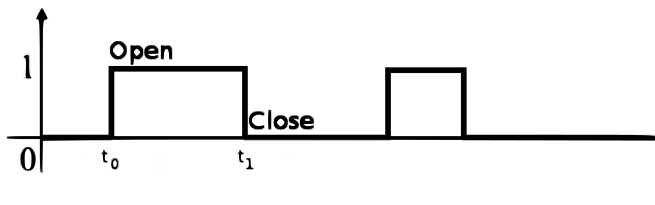
\includegraphics[width=\linewidth,totalheight=\textheight,keepaspectratio]{gfx/graph2.png}
      \caption{Sémantique des rôles.}
      \label{fig:semofroles}
\end{figure}

En pratique, pour fournir cette sémantique temporelle à l'application, 
l'implémentation d'un rôle doit être filtrée pour isoler les séquences de 
données atypiques (bruit). Par exemple, pour un rôle joué par un capteur de 
contact, s'il fournit deux valeurs true (ouverture) consécutives, l'implementation
filtrera habituellement la seconde valeur.

\section{Modèle d'infrastructure}\label{seq:fiabilite:model}
Les capteurs installés dans un domicile forment une infrastructure qui supporte 
les rôles requis par les applications déployées. 
La bonne implantation des rôles est critique pour la fiabilité de la 
sensibilité au contexte de cette infrastructure et donc des applications qui 
reposent sur cette infrastructure. 
Cette fiabilité va au-delà des tests unitaires de chaque rôle.

Pour adresser la fiabilité de l'infrastructure, nous proposons de construire un 
modèle de cette infrastructure qui peut être vérifié. Ce modèle ne prend pas 
uniquement en compte les rôles individuels, mais également leur conformité par 
des règles globales portant sur l'infrastructure de capteurs.

\subsection{Les évènements de rôle}\label{archi:algebra} 
La première étape pour expliciter le modèle d'infrastructure par un
ensemble de règles, est de délimiter le domaine des objets sur lesquels les 
règles pourront agir~: les évènements de rôle. Un évènement de rôle se compose de trois 
éléments~: (1) une interaction qui s'est produite (2) à une localisation donnée, 
(3) pendant une période de temps spécifique. Tout d'abord examinons la notion 
de période. Elle est définie en tant qu'intervalle délimité par deux horodatages. 
Ainsi~: 
\begin{displaymath}\label{archi:algebra:period1}
 \begin{array}{c} 
  Period = \mathds{N}^2\\
    \forall~p \in Period, p = <t_1, t_2>~and~t_1~<~t_2
 \end{array}
\end{displaymath}

Une période peut également être vue comme un ensemble de valeurs
de temps croissantes (ou d'instants), allant de $t_1$ à $t_2$, séparées chaque 
fois d'une seconde -- une granularité plus fine n'est pas 
nécessaire en pratique. Nous pouvons alors utiliser les opérations habituelles sur 
les ensembles pour opérer avec les périodes, comme $\subseteq, \supseteq$.

Enfin, un évènement de rôle est une interaction qui est arrivée pendant une 
période. L'ensemble d'interactions est définie par $Inter$ (\eg Présence, 
Ouverture, Utilisation). Un ensemble de localisations, $Loc$, spécifie 
les emplacements d'intérêt dans le domicile (\eg Cuisine, Salle de bain, Chambre). 
Les évènements de rôle sont donc définis comme suit.
\begin{displaymath}\label{archi:algebra:event}
  \begin{array}{c}
    e~\in~Event = Inter \times Loc \times Period \\
  \end{array}
\end{displaymath}

Lorsque l'infrastructure de capteurs surveille le domicile, elle produit des 
logs de données structurés en flux d'évènements de rôles, définis précédemment. 
Le log d'évènements de rôles est défini ainsi $log~\in~Log = \mathscr{P}(Event)$

\subsection{Formuler des règles}
Maintenant que les logs d'évènements de rôles sont définis et peuvent ainsi 
être manipulés, nous nous intéressons aux règles du modèle d'infrastructure. 
Ces règles sont exprimées par un ensemble de formules logiques dans le 
calcul de prédicats du premier ordre. Nous introduisons ces règles en examinant 
trois exemples de notre cas d'utilisation.

\myparagraph{Présence dans la cuisine.} Cette règle rend explicite la dépendance 
des capteurs dans la cuisine. En substance, nous voulons exprimer le fait que 
chaque interaction détectée, qui n'est pas un mouvement, doit être encadrée par 
une interaction de mouvement. Ce faisant, nous exprimons le fait que le capteur 
de mouvement dans la cuisine couvre toutes les autres interactions dans la 
cuisine (\eg porte de placard, machine à café). Une fois exprimée, cette 
sémantique assure la conformité des relevés de capteurs dans la cuisine.

Notre règle de présence dans la cuisine est définie ainsi~: 
\begin{displaymath}\label{archi:algebra:example}
  \begin{array}{c}
    \forall~<i, Kitchen, p>~\in~Log, i \neq Presence~ \Rightarrow \\
    ~~~~\exists~ <Presence, Kitchen, p'>~\in~Log,~p \subseteq p' 
  \end{array}
\end{displaymath}

\myparagraph{Portes restées ouvertes.} Nous supposons que dans un but 
d'assistance domiciliaire, une porte équipée d'un capteur de contact ne doit 
pas rester ouverte au-delà d'une certaine durée, notée $MAX$. Une telle règle 
s'applique typiquement sur la porte du frigidaire et sur la porte d'entrée 
parce que dans des conditions d'utilisation normales d'une maison, elles ne 
peuvent pas rester ouvertes très longtemps. La durée $MAX$ 
peut varier en fonction des préférences de l'utilisateur et du type de porte.

Cette règle est définie ainsi~:
\begin{displaymath}\label{archi:algebra:example2}
  \begin{array}{c}
    \forall~<Opening, l, p>~\in~Log \Rightarrow  \# p < MAX
  \end{array}
\end{displaymath}

Notons qu'une porte restée ouverte très longtemps peut être associée soit à un dysfonctionnement du 
capteur (comme pour les portes suscitées, de l'entrée ou du frigidaire), soit à un oubli de l'utilisateur de fermer la porte si celle-ci 
n'est pas surveillée par une application déclenchant une notification de 
sécurité. Par exemple, la porte du placard de notre cas d'utilisation est 
surveillée uniquement pour rappeler à l'utilisateur de préparer ses repas, et non pas pour 
lui rappeler qu'elle est restée ouverte. 

\myparagraph{Non omniprésence.} Certaines règles de conformité peuvent être 
spécifiques à un certain domaine d'application. Par exemple, 
nos recherches en informatique ubiquitaire sont principalement concentrées sur 
l'autonomie domiciliaire de personnes âgées vivant seules. Cette situation nous 
permet de définir la règle de conformité suivante: un rôle de présence ne peut 
pas être détecté simultanément à deux emplacements différents. La règle de non 
omniprésence est définie ainsi. 
\begin{displaymath}\label{archi:algebra:example3}
  \begin{array}{c}
    \forall~<Presence, l, p>~\in~Log \Rightarrow \\
     ~~~~\nexists~ <Presence, l', p'>~\in~Log,~l \neq l' \wedge ~p' \cap p \neq \emptyset
  \end{array}
\end{displaymath}

En pratique, définir des règles de conformité doit être associé à la fourniture d'instructions 
précises pour installer et positionner les capteurs dans le monde physique. 
Par exemple, la règle de présence dans la cuisine nécessite que la présence 
soit reconnue dans toute la cuisine. Une fois un domicile installé, les 
règles assurent la conformité entre l'installation et le modèle.

\section{Validation}\label{seq:fiabilite:validation}

Pour valider le concept de modèle d'infrastructure à base de règles,
nous présentons tout d'abord une architecture pour vérifier en continu qu'une installation 
est conforme à son modèle. Ensuite, nous décrivons une implantation de
cette architecture~; celle-ci nous a permis de valider l'approche expérimentalement.

\subsection{Architecture}
Globalement, l'architecture que nous proposons consiste à abstraire les lectures brutes de 
capteurs à travers une couche de rôles, alimentant à la fois les applications 
avec des valeurs de plus haut niveau, et les logs d'évènements de rôles utilisés par les 
règles de conformité du modèle d'infrastructure. Cette architecture est décrite 
en Figure~\ref{fig:archi}.

Les évènements de rôles sont traités simultanément par les applications et le 
module de vérification du modèle. Ce faisant, les règles de conformité peuvent être exécutées à la 
volée pour relever les erreurs quand elles apparaissent. Alternativement, les 
règles peuvent être exécutées hors ligne, sur des log déjà enregistrés, pour diagnostiquer des problèmes lorsque 
un opérateur est disponible pour de la maintenance.

\begin{figure}[!h]
  \centering
  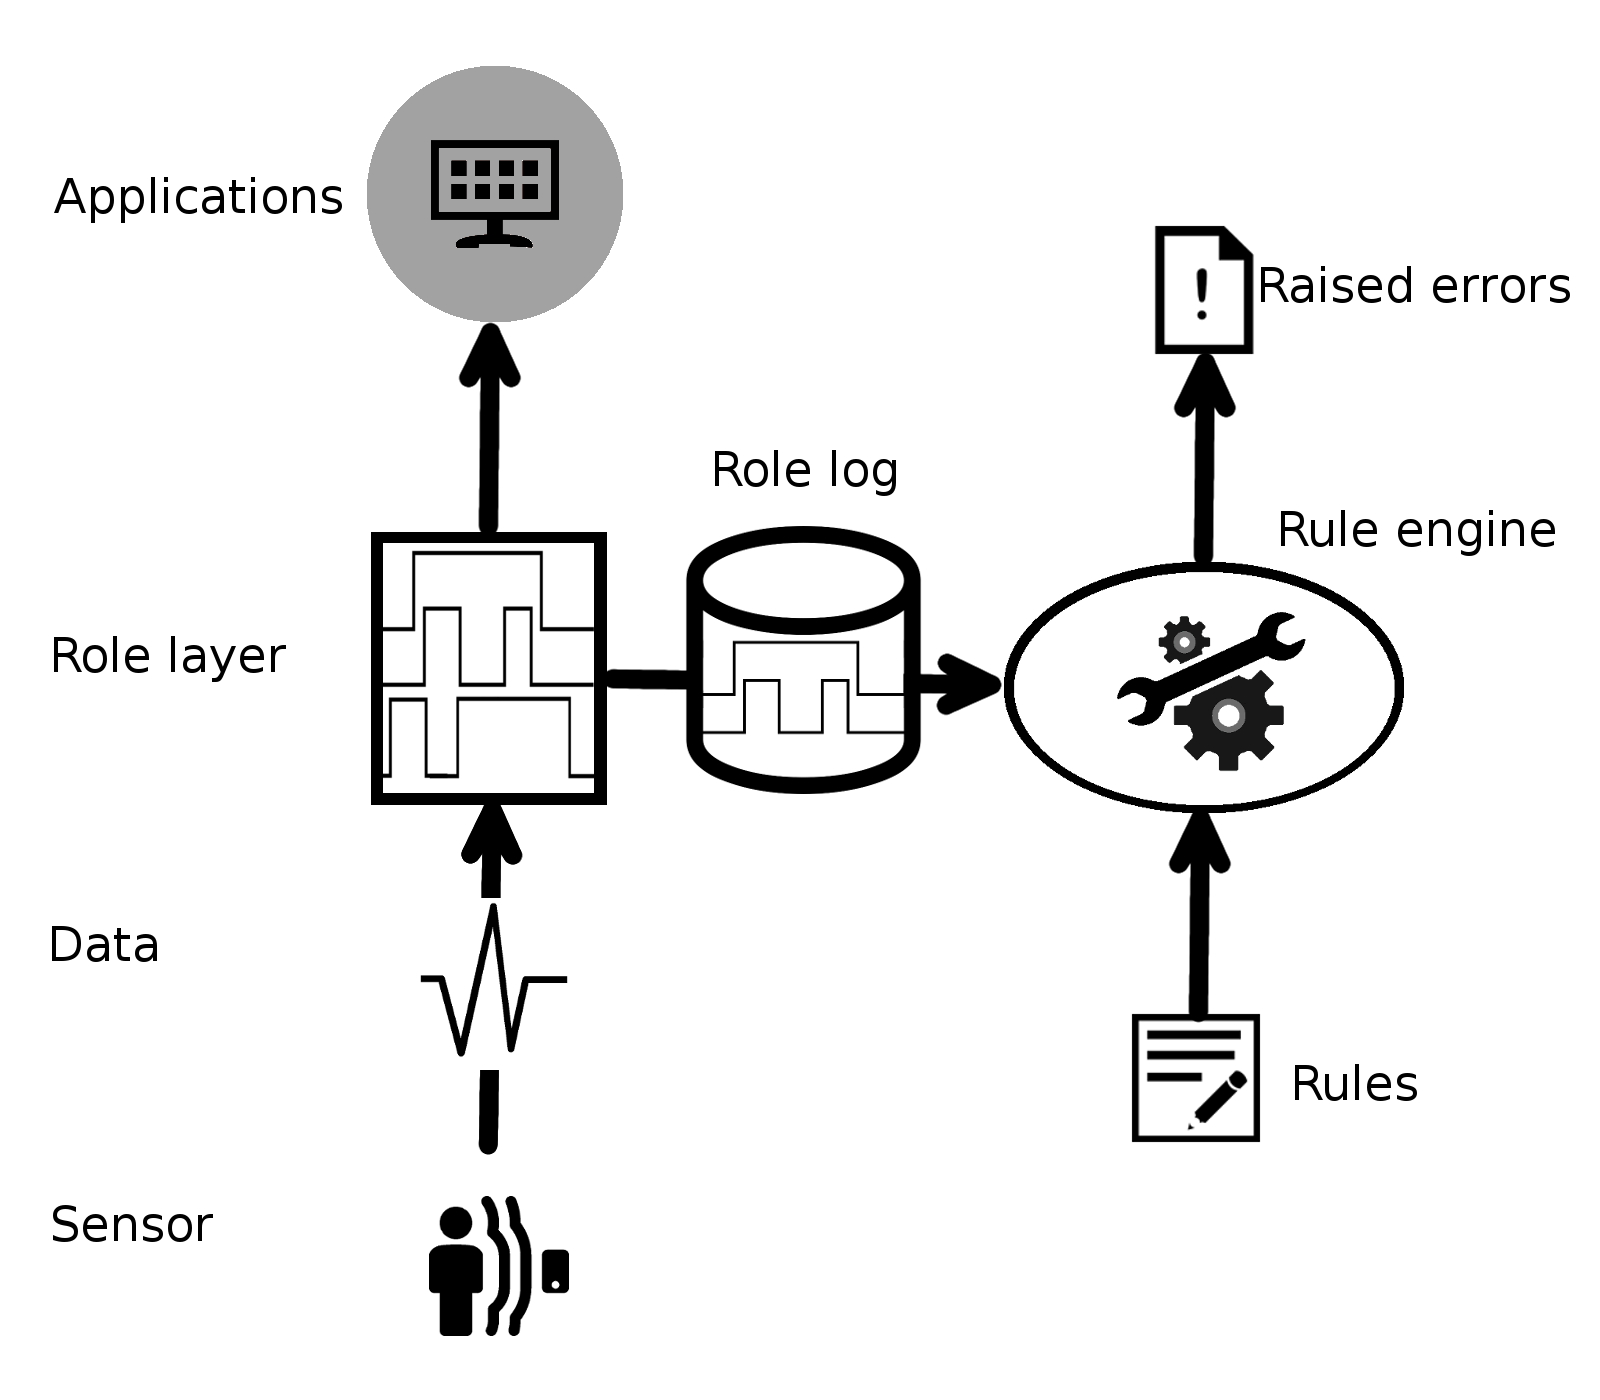
\includegraphics[width=\linewidth,totalheight=\textheight,keepaspectratio]{gfx/architecture.png}
  \caption{Architecture de notre approche de vérification continue d'une infrastructure par rapport à un modèle.}
  \label{fig:archi}
\end{figure}

Au-delà de la maintenance, les logs d'évènements de rôle peuvent aussi être 
précieux pour analyser l'évolution des activités quotidiennes des 
personnes âgées. En effet, ces logs permettent des analyses longitudinales qui 
peuvent, le cas échéant, révéler des dégradations du fonctionnement quotidien dues au 
vieillissement. Ces analyses permettent au professionnel d'adapter l'assistance 
en supprimant ou installant de nouvelles applications pour satisfaire l'évolution 
des besoins des utilisateurs. 

En outre, en faisant levier sur les logs d'évènements de rôle, la 
reconnaissance d'activités du quotidien peut être ajustée. Par exemple, le seuil 
de déclenchement des notifications peut être modifié pour prévenir la fatigue 
de l'utilisateur. De plus, ces logs peuvent servir pour rejouer des séquences 
d'interactions et déboguer des applications au comportement erroné.

\myparagraph{Règles.}
Les règles de conformité sont implantées sous la forme de prédicats Prolog, utilisant 
des opérateurs manipulant les évènements de rôles. 

\myparagraph{Analyseur de rôles.}
La plate-forme d'assistance utilisée pour valider notre approche ne fournissant 
pas la couche d'abstraction nécessaire pour produire les rôle, nous simulons 
cette couche dans notre implantation en utilisant un ``analyseur de rôles''. Ce 
composant construit un log d'évènements de rôles en transformant le log de 
lecture de capteurs et les informations associées (type de capteur, localisation, 
état et horodatage). Cet analyseur de rôle est implanté par un module C++.

\myparagraph{Moteur de règles.}
Ce module parcourt le log d'évènements de rôle produit par l'analyseur de rôles, 
et appelle un interpréteur Prolog pour exécuter chaque règle. De cette façon, 
quand une règle échoue, le moteur de règles identifie les évènements de rôle 
impliqués et produit une liste d'évènements de rôles non conformes avec les 
règles qu'ils ont fait échouer. Ce module est également implanté en C++. 
\newline

Le moteur de règles et l'analyseur de rôles totalisent plus de 2700 lignes de codes C++, 
pour transformer les données brutes de capteurs en évènements de rôles, et alimenter les règles en Prolog.

\subsection{L'expérimentation DomAssist}\label{seq:fiabilite:validation:domassist}
Le projet DomAssist\footnote{\url{http://phoenix.inria.fr/research-projects/homeassist}} 
vise à prolonger l'autonomie des personnes âgées dans leur propre 
domicile, en leur fournissant une plate-forme d'assistance domiciliaire avec des 
applications d'aide à la réalisation des activités quotidiennes. 
Des ergothérapeutes, psychologues et experts en vieillissement ont défini les 
activités à surveiller et l'ensemble des interactions à mesurer avec l'environnement.

Pour ce projet, deux types d'applications ont été définies~: (1) des applications 
pour surveiller les activités du quotidien et pour assister l'utilisateur quand elles 
n'ont pas été effectuées, et (2) des applications pour sécuriser le 
domicile ({\em e.g.,} porte d'entrée restée ouverte). Une première étude utilisateur a 
été conduite en recrutant 24 participants et en déployant à leur domicile notre 
plate-forme d'assistance domiciliaire pour une durée de neuf mois. Nous avons 
utilisé les données collectées durant cette première étude du projet DomAssist pour valider notre 
modèle d'infrastructure.

\subsection{Modèle}\label{validation:model} 
Les capteurs utilisés dans cette expérimentation permettent de mesurer douze 
interactions différentes avec l'environnement. Les interactions de présence sont 
mesurées avec des capteurs de mouvement, les ouvertures sont mesurées avec des 
capteurs de contact, et l'utilisation d'appareils électriques est mesurée avec 
des capteurs de consommation électrique. La configuration de DomAssist en terme 
de capteurs et leur rôles associés est résumée dans la Table~\ref{tab:domassist:role}.
\begin{table}[h!]
  \centering
  \begin{tabular}{|l|l|l|}
    \hline
    Room & Role & Sensor \\
    \hline
    \multirow{5}{*}{Kitchen} & Coffee maker in use & EM \\
    & Cabinet door open & CS \\
    & Fridge door open & CS \\
    & Microwave in use & EM \\
    & Presence & CS \\
    \hline
    \multirow{2}{*}{Entrance} & Door open & CS \\
    & Presence & MD \\
    \hline
    \multirow{2}{*}{Bathroom} & Shower in use & MD \\
    & Presence & MD \\
    \hline
    \multirow{2}{*}{Bedroom} & Dressing open & CS \\
    & Bedside lamp in use & EM \\
    & Presence & MD\\
    \hline
  \end{tabular}
\ \\ EM = Electric Meter, CS = Contact Sensor,\\ MD = Motion Detector.
  \caption{Rôles dans DomAssist.}
  \label{tab:domassist:role}
\end{table}

Pour des raisons pratiques, notre approche n'a pas pu être déployée au commencement 
de l'expérimentation DomAssist. 
% Nous avons donc appliqué notre 
% approche a posteriori. 
Notre modèle a donc été appliqué rétrospectivement pour 
vérifier la conformité du domicile de chaque participant en exécutant les règles 
sur les logs accumulés durant l'expérimentation.

En étudiant les conditions de l'expérimentation et nos rôles, nous avons 
spécifié les règles de conformité qui rendent explicites les conditions de 
l'étude~: les participants vivent seuls (règle de non omniprésence) 
et certaines interactions avec l'environnement doivent suivre un motif spécifique 
(porte restée ouverte). D'autres règles ne dépendent pas de l'objectif de l'étude 
et peuvent être généralisées. La règle d'inclusion de présence et ses 
raffinements (intersection de présence et besoin de présence) en sont des illustrations.
Examinons maintenant ces règles.

\myparagraph{Non omniprésence.}
Cette règle assure qu'un rôle de présence n'est pas détecté simultanément à deux 
localisations différentes. En pratique, en fonction de la réactivité des capteurs 
de mouvements utilisés pour la détection de présence, quelques brefs chevauchements 
peuvent survenir et doivent être ignorés. Typiquement, un détecteur de présence 
signale une absence avec une latence. Cette latence rend possible la
détection simultanée  de l'utilisateur dans deux pièces pendant quelques instants.

\myparagraph{Porte restée ouverte.}
Cette règle assure que la période d'un rôle d'ouverture de porte ne dure pas 
plus d'un certain temps (trois heures dans notre configuration). 
Notons que cette règle est exécutée sur les logs d'évènements, en complément
d'autres applications d'assistance qui peuvent réagir aussi 
à une telle situation. Par exemple, DomAssist inclut une application qui 
surveille la porte d'entrée. Cette application notifie l'utilisateur quand la porte est restée 
ouverte, sans surveillance pendant quelques minutes (la durée est configurée 
en fonction de l'utilisateur). Aussi, quand elle est appliquée aux logs 
de notre étude, cette règle détecte dans la plupart des cas des problèmes 
d'installation. 
% \cc je ne comprends pas la phrase suivante. Remplace "cela" par un mot et relis l'ensemble du paragraphe.
% Cependant, cette règle reste vrai même pour des portes non surveillées par des 
% applications de sécurité. 
Cette situation concerne également les portes non surveillées par des 
applications de sécurité (telle une porte de placard), ce qui s'explique par le fait que
les participants sont routinisés dans leurs
activités~\paulcite{bergua2013restriction} et n'ont pas déclinés  
cognitivement de façon significative durant l'étude.

\myparagraph{Inclusion de présence.}
Chaque pièce pour laquelle une interaction doit être détectée est équipée avec 
un détecteur de mouvement. Par conséquent, nous avons généralisé la règle de 
présence dans la cuisine à toutes les pièces~: toute interaction, qui n'est pas 
une présence, à une localisation donnée, doit être inclue dans un rôle de 
présence à la même localisation. 

\myparagraph{Intersection de présence.}
L'inclusion de présence peut être trop contraignante pour s'appliquer à 
certaines situations. Parfois, nous devons simplement nous assurer que la 
présence et d'autres interactions ont une intersections non nulle quand elle 
sont situées dans la même pièce. Une telle règle s'applique dans l'entrée du 
domicile, équipée d'un capteur de contact sur la porte d'entrée et un capteur 
de mouvement dans l'entrée (zone située à l'intérieur du domicile). 
En effet, si l'utilisateur ouvre la porte, que ce soit 
depuis l'extérieur ou depuis l'intérieur, les rôles de présence et d'ouverture ont une 
période de temps durant laquelle leur intersection est non-nulle.

\myparagraph{Besoin de présence.}
Pour s'assurer que le détecteur de mouvement est toujours actif même si il est 
mal positionné, nous introduisons la règle suivante~: chaque rôle, qui n'est pas 
une présence, doit être accompagné d'un évènement de rôle présence à la même 
localisation. Cette présence doit arriver au même moment plus ou moins dix minutes. 
Cette règle rend explicite le fait que le capteur de mouvement est toujours 
couplé avec un ou plusieurs autres capteurs dans notre configuration. La 
violation de cette règle indique principalement que le capteur de mouvement 
ne fonctionne pas correctement, probablement car il est toujours enregistré dans le système, 
mais n'émet plus aucune donnée.

\subsection{Méthodologie}\label{validation:methodology}
Nous avons collecté les logs des capteurs placés dans les habitations des 24 participants à 
l'étude. Ces participants sont âgés de 80 ans en moyenne et habitent seuls. Les 
données collectées couvrent une période de neuf mois. Cependant, des problèmes 
techniques (\eg accès internet, passerelle domotique, serveur) nous ont poussé 
à ignorer certaines périodes de temps~; ces problèmes peuvent être directement 
détectés par la plate-forme. Les logs de l'expérimentation ont également 
été nettoyés en éliminant les évènements de rôle non conformes 
pouvant être détectés par un mécanisme de tolérance aux fautes détectant 
les fautes de capteurs et de réseau, selon la classification définie 
par Chetan~\etal~\parencite{chetan2005toward}.
% simple système de surveillance de type
% heartbeat. 
% \cc mettre une citation et mentionner que c'est un mecanisme de tolerance aux fautes (a verifier)
%En effet, 
Par exemple, l'absence de signal de heartbeat, normalement émis par tout capteur, 
est détectée par les couches basses de la plate-forme et signalée comme un échec 
de communication avec le capteur.

Nous avons examiné le plan du domicile de chaque participant, spécifiant le placement 
et le positionnement des capteurs. Ce document a été utilisé pour 
diagnostiquer les problèmes quand des violations de conformités sont arrivées dans 
les logs. D'autres ressources ont été également disponibles pour diagnostiquer 
les violations, telles que les fichiers de suivi des interventions remplies par les 
professionnels chargés de faire passer des questionnaires à chaque participant
durant l'étude.

\subsection{Résultats expérimentaux}\label{validation:results}
Le modèle défini pour DomAssist permet de lever deux types 
d'anomalies~: (1) {\em les non-conformités permanentes} -- elles font réfèrence à une règle 
systématiquement transgressée, indiquant des non concordances permanentes entre 
l'infrastructure et le modèle~; (2) {\em les non-conformités émergentes}
-- elles correspondent à une règle qui est vérifiée la plupart du temps, mais échoue 
ponctuellement.

\myparagraph{Non-conformités permanentes.}
Dans un domicile, l'interaction d'ouverture est détectée pour la porte du 
placard de la cuisine, mais les règles {\em inclusion de présence} et 
{\em intersection de présence} échouent systématiquement. Cependant, 
la règle de {\em besoin de présence} n'échoue jamais, indiquant que la porte de 
placard est ouverte mais jamais couverte, ni même en intersection avec une interaction de présence dans la 
cuisine~; la présence est donc détectée à des moments proches mais disjoints de
l'interaction d'ouverture. La consultation des documents relatifs à cette 
installation ont montré que ce placard n'est pas localisé dans la cuisine mais 
dans une pièce attenante, comme montré en Figure~\ref{fig:map}. Cette situation 
montre un problème dans la définition du modèle pour cette
installation. Par conséquent, nous avons modifié le modèle de cette installation en y supprimant 
les règles d'inclusion de présence et d'intersection de présence. Nous
les avons remplacées par la règle besoin de présence, mieux adaptée à cette configuration.

Dans ce même domicile, un autre problème à été identifié~: la règle 
{\em inclusion de présence} échoue systématiquement sur le rôle d'ouverture du 
frigidaire, mais l'{\em intersection de présence} n'échoue jamais. Bien que le 
frigidaire soit localisé dans la cuisine, le capteur de mouvement utilisé pour 
mesuré la présence dans la cuisine, n'a pas été positionné pour couvrir 
l'ensemble de la cuisine, comme montré en Figure~\ref{fig:map}. 
Ce problème provient dans ce cas d'une erreur à l'installation et la solution
consiste simplement à changer le positionnement du capteur de mouvement. 

Nous avons observé la même configuration du placard de la cuisine situé en 
dehors de la cuisine, dans deux autres domiciles.

Généralement, ces types de problèmes surviennent quand la plate-forme d'assistance est 
déployée à large échelle. Dans ce contexte, les installations sont faites par 
un professionnel, et non par les chercheurs qui ont conçu la
plate-forme et qui possèdent un savoir implicite sur la bonne manière de déployer. Dans notre cas, 
même pour 24 domiciles, quelques installations ont été faites par des membres 
n'ayant pas ce savoir, et donc n'ont pas pu se conformés à certaines règles implicites.

\begin{figure}[!h]
  \centering
      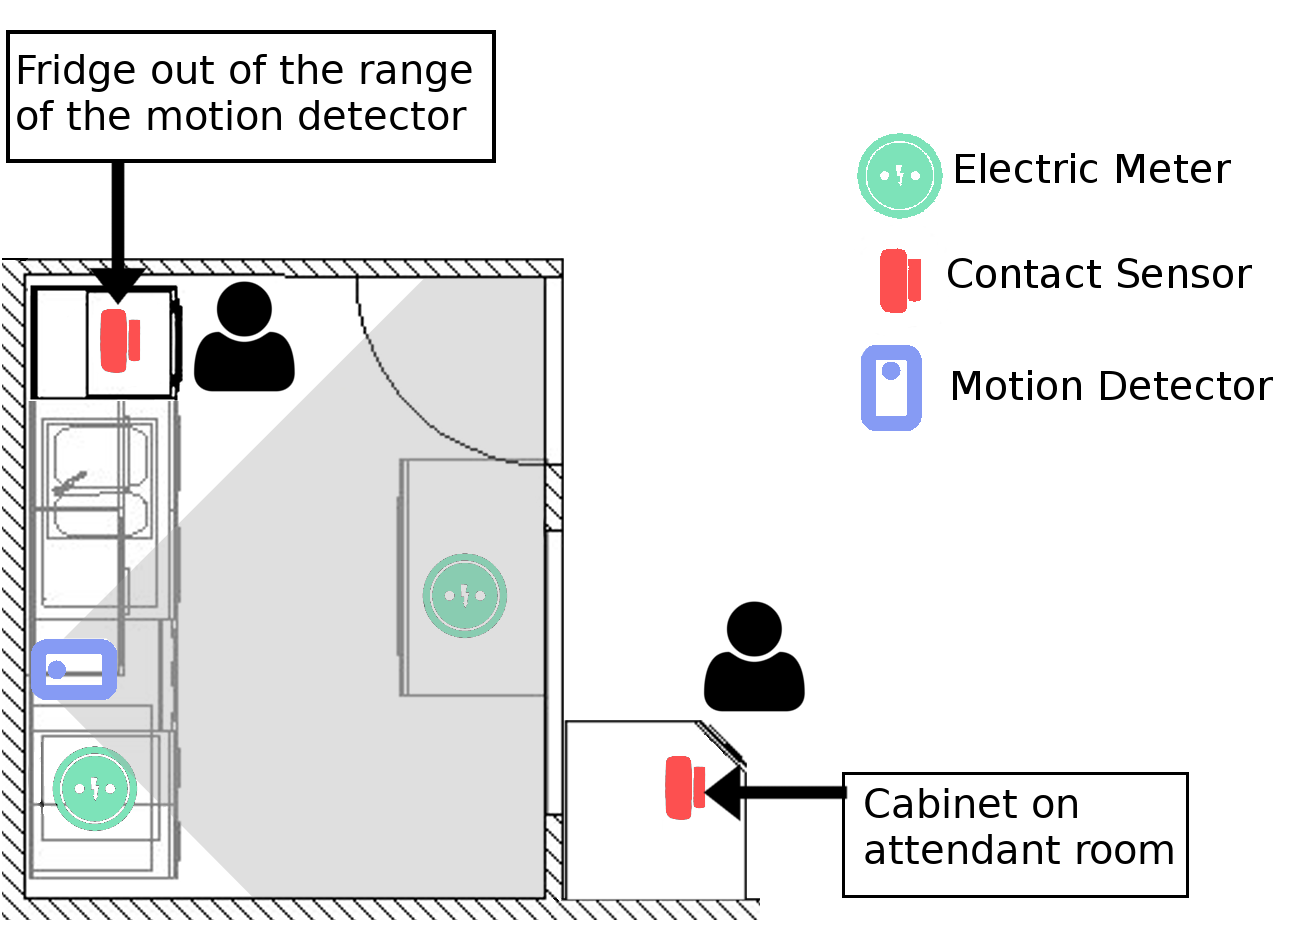
\includegraphics[width=\linewidth,totalheight=\textheight,keepaspectratio]{gfx/nconf2.png}
      \caption{Illustration de problèmes d'installation.}
      \label{fig:map}
\end{figure}

Si notre outil avait été utilisé dès la phase de déploiement, il aurait été 
possible de détecter les anomalies d'installation dès le départ, pendant 
l'installation ou dans les premiers jours d'exploitation. Par ailleurs, une 
fois déployées, des règles supplémentaires peuvent affiner les modèle pour 
prendre en compte des spécifications imprévues (\eg cuisine en forme de L). 
Une fois l'installation ou le modèle affiné, notre approche contribue à la détection 
d'anomalies au quotidien, en une période de fonctionnement normal.

\myparagraph{Non-conformités émergentes.}
Un motif de non concordance a été observé dans cinq domiciles à différentes 
périodes de temps. Pendant plusieurs jours, la règle {\em inclusion de présence} 
a été enfreinte par une absence de présence dans la cuisine causée par un 
capteur de mouvement qui dysfonctionnait. Dans chacun des cas, les règles 
d'{\em intersection de présence} et de {\em besoin de présence} étaient 
également transgressée durant ces périodes. Cette dernière règle montre 
qu'aucun rôle de présence n'a été reconnu durant les 20 minutes entourant cette 
violation. Les résultats de ces règles fournissent de précieuses informations 
pour trouver la cause des dysfonctionnement relevés. Il est alors raisonnable de 
supposer que la cause de cet échec des règles est un dysfonctionnement temporaire 
du rôle de présence. Nous pouvons supposer que le capteur de mouvement a pu être obstrué 
ou déplacé. 

Une situation similaire est arrivée dans l'entrée de deux autres domiciles~: la 
porte a parfois été ouverte, sans qu'aucune présence n'ait été détectée.

La {\em porte restée ouverte} a été observée dans quatre domiciles à différents 
endroits comme le frigidaire, le placard de la cuisine ou la penderie (\ie la 
porte est restée ouverte plus de trois heures). D'après les fichiers de suivi 
des interventions de l'expérimentation, les utilisateurs concernés ont été 
questionnés après quelques jours sur les comportements erronés des applications 
reposant sur ces interactions. Ils ont indiqué que les capteurs de contact 
étaient tombés. Les installations ont alors été réparées par les techniciens 
chargés des interventions. Notre modèle, si il avait été disponible durant 
cette expérimentation aurait permis de rapporter ces incidents, et de les 
solutionner plus rapidement. Cette réactivité est indispensable pour la pertinence 
des résultats des application sensibles au contexte. Elle fait toute la différence 
entre une application utile et une application qui harcèle l'utilisateur avec 
des notifications non pertinentes.

\section{Discussion}\label{sec:discussion}
Un modèle explicite d'une infrastructure est capable de détecter les 
dysfonctionnements du systèmes durant la phase d'installation ou pendant 
l'exploitation normale. Comme suggéré par certains de nos exemples, une fois 
une erreur détectée, quelques techniques de diagnostic peuvent être utilisées 
pour identifier les rôles qui sont la source de l'erreur.  

Premièrement, si plusieurs règles sont violées en même temps, et que ces règles 
concernent des ensembles de capteurs qui se chevauchent, il est alors probable 
que le rôle à la source de cette erreur soit à rechercher à l'intersection de 
ces ensembles. Par exemple, quand la règle {\em intersection de présence} 
échoue en même temps pour le rôle présence dans la cuisine et pour différentes 
interactions qui ne sont pas des présences (frigidaire, placard, \etc), 
%on peut 
%supposer que 
le rôle défaillant est 
probablement 
la présence 
dans la cuisine. 

Deuxièmement, concevoir une version raffinée d'une règle qui vérifie un ensemble 
de capteurs (ou est un sous-ensemble de la règle de base) peut s'avérer utile 
pour diriger la recherche d'un rôle défaillant ou d'un capteur qui dysfonctionne. 
Cette idée est illustrée dans notre modèle pour DomAssist. Il y a une chaîne 
de trois règles $R_i$ avec des conditions de moins en moins précises~:
{\em inclusion de présence}, {\em intersection de présence} et 
{\em besoin de présence}. Toutes ces règles sont du type 
$p \rightarrow q_i$ pour $(i=1..3)$ où le postulat $p$ est identique, mais la 
conclusion $q_i$ est de plus en plus faible. Il y a une implication tout au long 
de la chaîne, $R_1 \rightarrow R_2 \rightarrow R_3$~; ou inversement, quand une 
des règles échoue, les règles les plus fortes échouent également. Basé sur 
l'analyse des règles, nous pouvons définir un arbre de décision comme celui en 
Figure~\ref{fig:bdd} pour aider au diagnostic.

\begin{figure}[!h]
  \centering
      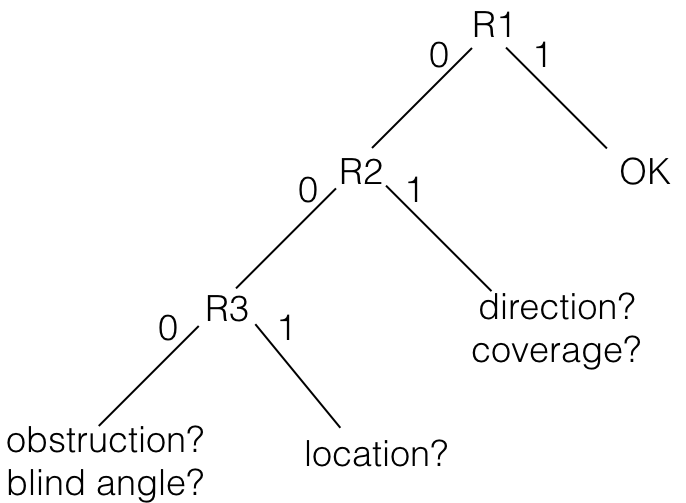
\includegraphics[scale=0.3]{gfx/bdd.png}
      \caption{Arbre de décision binaire aidant au diagnostic de la source d'une défaillance.}
      \label{fig:bdd}
\end{figure}

L'utilité de notre approche pour assurer continuellement la conformité d'une 
infrastructure va au-delà de la détection d'infrastructures défaillantes. 
Par exemple, un modèle d'infrastructure pourrait fournir un modèle de référence pour des applications 
disponibles dans un catalogue en ligne de type Appstore~: une application pourrait 
être installée uniquement lorsqu'elle est conforme au modèle d'infrastructure. 
En pratique, ce filtrage des applications au moment de l'installation pourrait remplacer
un certain nombre de tests qui sont nécessaires aujourd'hui pour chaque application déployée sur une installation
donnée, pourvu que le modèle couvre toutes les hypothèses requises par les applications.

\section{Conclusion}\label{sec:futurework}
Nous avons montré que les applications sensibles au contexte reposent 
fréquemment sur des suppositions implicites concernant l'infrastructure de capteurs. Ces 
suppositions se traduisent généralement en terme de programmation par des instructions conditionnelles qui 
polluent le code avec des préoccupations non fonctionnelles. Cette approche de programmation
défensive peut être évitée en exprimant ces suppositions, non pas dans le code 
des applications, mais en les factorisant dans un modèle explicite 
d'infrastructure de capteurs. Non seulement la violation d'une règle
du modèle d'infrastructure
permet d'alerter rapidement sur un dysfonctionnement de
l'installation, mais cette situation
contribue également à diagnostiquer le problème. 
Une telle approche permet de s'assurer de la fiabilité de la sensibilité au 
contexte des applications d'assistance domiciliaire. De plus, la définition du 
modèle permet de fourmuler des instructions détaillées quant à l'installation 
des capteurs dans le domicile, rendant ce dernier sensible au contexte.


% Our approach has been implemented in the context of an assisted living platform, running a set of applications dedicated to assist senior users. Our tool was applied to real sensor data collected during a 9-month field study, consisting of 24 participants aged 80 on average. The results show that some latent installation mistakes could have been found at installation time, using our model. Furthermore, several sensor problems that occurred during operation could have been detected on the fly and repaired more promptly to ensure the reliability of context-awareness applications.

% In future work, we will apply our method in a larger deployment consisting in hundreds of installations. This setting will allow us to quantify in more detail the improved reactivity in detecting emerging infrastructure issues, remotely diagnosing the underlying failure, and repairing the platform on-site. Another future work will consist of proposing log visualisation techniques and tools that contribute to identify new rules for the model by recognizing regular event patterns and anomalies. 